\hypertarget{modelling-reactive-behavior-notation}{%
\section{Modelling Reactive Behavior
Notation}\label{modelling-reactive-behavior-notation}}

\hypertarget{finite-state-machine}{%
\subsection{Finite State Machine}\label{finite-state-machine}}

\emph{A model of state dependent behaviour}\\
In a finite state machine, the event and the action are in the opposite
direction of a technical process. The reason here is that the events of
the technical process is the input for the finite state machine.

\begin{figure}[H]
\centering
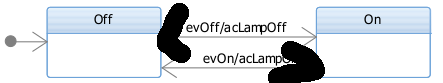
\includegraphics[width=0.5\textwidth]{figures/fsm.png}
\caption{Finite state machine}
\end{figure}

\hypertarget{uml-state-diagrams}{%
\subsubsection{UML State-Diagrams}\label{uml-state-diagrams}}

\hypertarget{time-events}{%
\paragraph{Time Events}\label{time-events}}

\begin{itemize}
\tightlist
\item
  Time Events can be used to trigger Transitions
\item
  Time Events occur a specified time after entering a certain state
\end{itemize}

Notation:\\
- Rhapsody: tm(timeUnits) (in this lecture: timeUnit = 1 ms) - Standard
UML: after(500ms)

\begin{figure}[H]
\centering
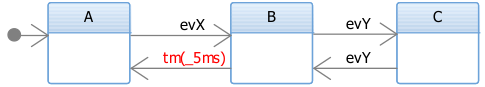
\includegraphics[width=0.5\textwidth]{figures/fsmTimeEvent.png}
\caption{Time Event FSM}
\end{figure}

\hypertarget{operation-calls-in-actions}{%
\paragraph{Operation Calls in
Actions}\label{operation-calls-in-actions}}

\begin{figure}[H]
\centering
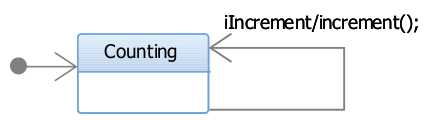
\includegraphics[width=0.5\textwidth]{figures/fsmOperationCall.png}
\caption{Operation Calls}
\end{figure}

\clearpage
\hypertarget{entry-and-exit-actions}{%
\paragraph{Entry and Exit Actions}\label{entry-and-exit-actions}}

\begin{itemize}
\tightlist
\item
  Entry Actions are executed every time a State is entered
\item
  Exit Actions are executed every time a State left
\end{itemize}

\begin{figure}[H]
\centering
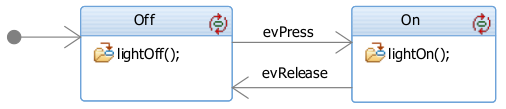
\includegraphics[width=0.5\textwidth]{figures/fsmEntryExitAction.png}
\caption{Entry and Exit Actions}
\end{figure}

\hypertarget{internal-transition}{%
\paragraph{Internal Transition}\label{internal-transition}}

\begin{figure}[H]
\centering
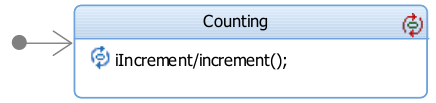
\includegraphics[width=0.5\textwidth]{figures/fsmInternalTransition.png}
\caption{Internal Transition}
\end{figure}

\hypertarget{completion-transitions}{%
\paragraph{Completion transitions}\label{completion-transitions}}

\begin{itemize}
\tightlist
\item
  Also called null transitions
\item
  Have no trigger
\item
  Are executed at the after a state is entered and all entry actions are
  executed (and Out-Pulses are sent see below)
\item
  Belong to run-to-completion step (see below) of the triggering
  transition
\item
  Can have guards (see below)
\item
  Can have actions
\item
  With more completion transitions, guards are needed to make them
  deterministic
\end{itemize}

\hypertarget{guards}{%
\paragraph{Guards}\label{guards}}

A guard is a boolean condition that can be assigned to a transition

\begin{figure}[H]
\centering
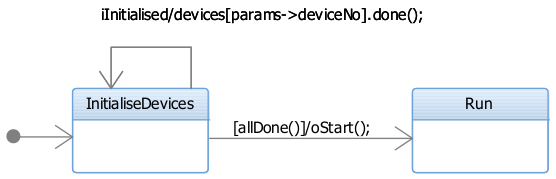
\includegraphics[width=0.5\textwidth]{figures/fsmGuard.png}
\caption{FSM Guards}
\end{figure}

\clearpage
\hypertarget{nested-states}{%
\paragraph{Nested States}\label{nested-states}}

Finite state machines can be nested.

\begin{figure}[H]
\centering
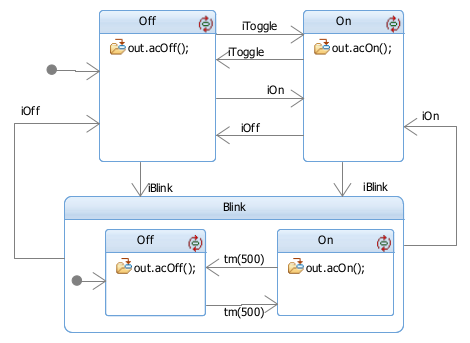
\includegraphics[width=0.5\textwidth]{figures/fsmNested.png}
\caption{FSM nested}
\end{figure}

\hypertarget{history}{%
\paragraph{History}\label{history}}

The history means, that I enter the same state into the FSM as I was
when I left the FSM.

\begin{figure}[H]
\centering
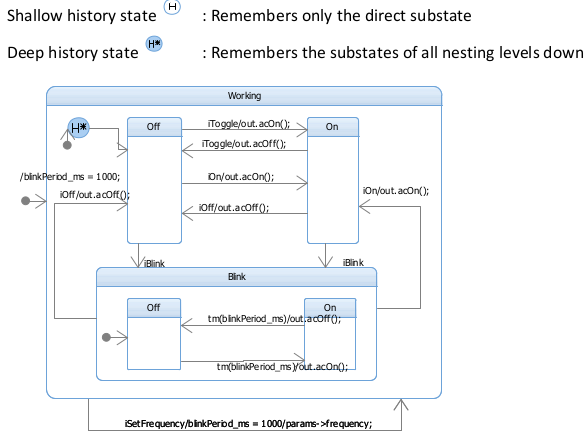
\includegraphics[width=0.5\textwidth]{figures/fsmHistory.png}
\caption{FSM History}
\end{figure}

\clearpage
\hypertarget{junction-state}{%
\paragraph{Junction State}\label{junction-state}}

Chains transition segments into a single transition or the other one
outgoing transition in multiple outgoing transitions.

\begin{figure}[H]
\centering
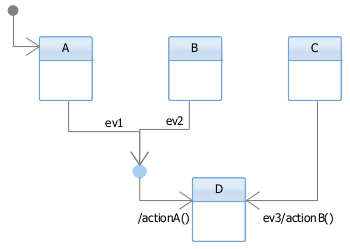
\includegraphics[width=0.5\textwidth]{figures/fsmJunctionState.png}
\caption{FSM Junction State}
\end{figure}

\subsection{CIRO (Communicating Interacting Reactive-Objects)}

\begin{itemize}
\tightlist
\item
  UML Extension
\item
  To model reactive systems
\item
  Asynchronous communication with (event-, action-, communication-)
  messages
\item
  Synchronous interaction between reactive-objects (see below)
\item
  Code-generation possible
\end{itemize}

\hypertarget{meta-model-not-important}{%
\subsubsection{Meta-model (not
important)}\label{meta-model-not-important}}

\begin{itemize}
\tightlist
\item
  Meta-Model: a model of models
\item
  Meta-Model defines:

  \begin{itemize}
  \tightlist
  \item
    the elements of a modelling language
  \item
    the set of potential models (syntactically correct models)
  \item
    the semantics (i.e.~the meaning) of the model elements
  \end{itemize}
\end{itemize}

\clearpage
\hypertarget{reactive-system}{%
\subsubsection{Reactive-System}\label{reactive-system}}

A reactive system is the sum (logical aggregate) of all
reactive-machines of an Embedded-System. - Input: Event-Messages -
Output: Action-Messages

\begin{figure}[H]
\centering
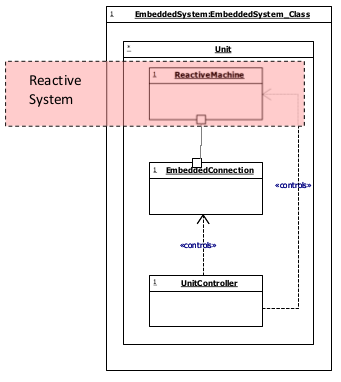
\includegraphics[width=0.5\textwidth]{figures/reactiveSystemOverview.png}
\caption{Reactive System Overview}
\end{figure}

\begin{itemize}
\tightlist
\item
  The \textbf{Reactive Machine} or \textbf{Reactive Object} is one
  component of a cluster. In the vessel e.g.~the pump.
\item
  The \textbf{Reactive Cluster} is one cluster in a reactive system,
  e.g.~the cluster of different components in the vessel.
\item
  If there would be a system with multiple clusters, all clusters
  together would be the \textbf{reactive system}.
\end{itemize}

\begin{figure}[H]
\centering
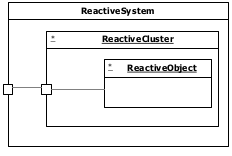
\includegraphics[width=0.5\textwidth]{figures/reactiveSystemCluster.png}
\caption{Reactive System Cluster}
\end{figure}

\hypertarget{reactive-cluster}{%
\subsubsection{Reactive-Cluster}\label{reactive-cluster}}

Reacts to event-messages and generates action-messages. A group of
cooperation objects which are interacting with each other. Within a
cluster Reactive-Objects cooperate using 3 different synchronous
interaction mechanisms - Pulse-Cast - State-Inspection - Mode-Control

\hypertarget{reactive-object}{%
\subsubsection{Reactive-Object}\label{reactive-object}}

\begin{itemize}
\tightlist
\item
  Component of a Reactive-Cluster
\item
  Defines a finite state machine (FSM) or extend finite state machine
  (see below)
\item
  Interacts synchronously with other Reactive-Objects within the same
  cluster
\item
  Communicates indirectly via cluster-Button: Mode normal ports with the
  outside world
\end{itemize}

\hypertarget{interaction-mechanisms}{%
\subsubsection{Interaction mechanisms}\label{interaction-mechanisms}}

\begin{itemize}
\tightlist
\item
  Pulse-Cast

  \begin{itemize}
  \tightlist
  \item
    Multi-cast, one sender, many receivers
  \item
    In-Pulse

    \begin{itemize}
    \tightlist
    \item
      Input to state-machine
    \item
      Triggers state-transition
    \end{itemize}
  \item
    Out-Pulse

    \begin{itemize}
    \tightlist
    \item
      Output of state-machine
    \item
      Generates in-pulse to receiver
    \end{itemize}
  \end{itemize}
\item
  State-Inspection

  \begin{itemize}
  \tightlist
  \item
    Enables case differentiation on transitions
  \end{itemize}
\item
  Mode-Control

  \begin{itemize}
  \tightlist
  \item
    Determination of the active mode
  \end{itemize}
\end{itemize}

\clearpage